\documentclass{article}
\usepackage{graphicx}
\usepackage{fullpage}
\usepackage{amsmath}
\usepackage{hyperref}
\usepackage{tikz}
\usepackage[]{algorithm2e}

\usetikzlibrary{decorations.pathreplacing}

\title{Parallel domain decomposition in 2D}
\author{Gavin Stewart and Sanchit Chaturvedi}

\begin{document}
	\maketitle
	
	\section{Introduction}
	
	Elliptic problems are important in applied and mathematical physics.  The Poisson equation 
	\begin{equation}
	-\Delta u = f
	\end{equation} describes the voltage \(u\) due to a charge distribution with density \(f\)%REF
	, as well as describing the pressure in incompressible fluid flow \cite{Marshall97}. The Helmholtz equation
	\begin{equation}
	(-\Delta u + k^2)u = f
	\end{equation} 
	describes the propagation of electromagnetic or acoustic waves \cite{Fairweather03}.
	
	For large scale problems, it is desirable to parallelize the computation of solutions.  This is difficult for elliptic problems due to the strong coupling between unknowns when \(u\) is computed through finite difference or finite element methods.  Domain decomposition methods split the computational domain into several regions (which may or may not overlap), compute an estimate of the solution on each  subdomain, and then combine the solutions on each subdomain to get an estimate of the new solution.  The choice of boundary conditions for the subdomains varies between different methods \cite{Dolean15}; we will use a method with Dirichlet boundary conditions.
	
	In this report, we give a parallel algorithm for solving the Poisson equation by domain decomposition.  The layout of the report is as follows: in section 2, we will describe the domain decomposition algorithm in detail.  In section 3, we will give weak and strong scaling results for an implementation of the algorithm with \(0\) overlap.  In section 4, we give an explanation for the slow convergence of the method, and suggest possible improvements to speed up the method.  Finally, section 5 gives an account of both authors' contributions to the project.
	
	\section{The algorithm}
	
	Domain decomposition can be implemented in many forms.  In our project, we used a restricted additive Schwarz method (chapter 1 of \cite{Dolean15}).  We will first summarize the algorithm in its continuous form, then provide more detail on our parallel implementation.
	
	\subsection{The continuous algorithm}
	
	Suppose \(\Omega = \Omega_1 \cup \Omega_2 \cdots \Omega_N\), and let \(u^0\) be a function defined on \(\Omega\).  Let \(\xi_i\) be a partition of unity on \(\Omega\): that is \(\xi_i(x) = 0\) for \(x \not\in \Omega_i\) and \(\sum_{i=1}^N \xi_i(x) = 1\) for every \(x \in \Omega\).
	
	The iteration is as follows.  Suppose the \(n\)th iterate of the solution, \(u^n\), is known.  Then, we define the residual to be \(r^n = \Delta u^n + f\).  If \(u^n\) is an exact solution, then \(r^n = 0\).  Otherwise, we want to compute a correction \(v^n\) such that \(-\Delta v^n = r^n\), since then \(u^{n+1} = v^n + u^n\) will solve the Poisson equation exactly.  
	
	We attempt to approximate \(v^n\) using local solutions to the problem.  Let \(r^n_i\) be the restriction of \(r^n\) to \(\Omega_i\), and define \(v^n_i\) to be the solution to 
	\begin{equation}
	\begin{split}
	-\Delta v^n_i = r^n_i\quad \text{ in } \Omega_i\\
	v^n_i = 0 \quad \text{ on } \partial\Omega_i
	\end{split}
	\end{equation}
	
	Finally, let \(v^n = \sum_{i=1}^N\xi_iv^n_i\), and define \(u^{n+1} = u^n + v^n\).  It can be shown that for domains with overlap, the solutions \(u^{n+1}\) converge to the true solution \cite{Dolean15}.
	
	\subsection{The parallel implementation}
	
	For the parallel implementation, let \(\Omega = (0,1)\times(0,1)\), and let the \(\Omega_1, \cdots, \Omega_{k^2}\) be a checkerboard tiling of \(\Omega\) (Figure~\ref{fig:decomp_pic}).  Place evenly spaced points in the domain in a \(kn \times kn\) grid, so each domain has \(n \times n\) gridpoints.  The algorithm is given in Algorithm~\ref{alg:RAS}.  
	
	\begin{figure}
		\begin{center}
			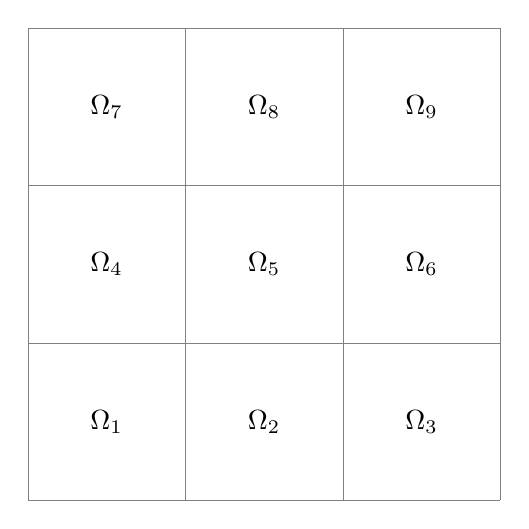
\begin{tikzpicture}[scale=2]
			\draw[help lines] (0,0) grid (3,3);
			\foreach \x in {0,1,2}
			\foreach \y in {0,1,2}
			{\pgfmathtruncatemacro{\label}{1+ \x + 3 *  \y}
				\node (\x\y) at (0.5+\x,0.5+\y) {$\Omega_\label$};}
			\end{tikzpicture}
		\end{center}
		\caption{\label{fig:decomp_pic} The decomposition of the domain for \(k = 3\).}
	\end{figure}
	
	\begin{algorithm}[H]
		\KwIn{An initial solution \(u^0\), the forcing function \(f\), and a tolerance \(\epsilon\)}
		\KwResult{An estimate of the solution \(u\)}
		Each processor reads in its section of the global solution \(u_i\)
		Each processor computes its local residual \(r_i\)\;
		All processors compute the norm of the global residual, \(\lVert r \rVert\)\;
		\While{\(\lVert r \rVert \ge \epsilon\)}{
			Each processor computes an update \(v_i\) as \(A_iv_i = u_i\)\;
			Each processor computes its local residual \(r_i\)\;
			All processors compute the norm of the global residual, \(\lVert r \rVert\)\;
		}
		\caption{\label{alg:RAS}The discrete RAS algorithm.}
	\end{algorithm}
	
	The matrix \(A_i\) is the usual matrix describing the Laplace equation with the 5-point stencil, 
	\begin{equation}
	A_i = \frac{1}{h^2}\begin{bmatrix}
	4 & -1  &    & -1 &    &    &    &    &   \\
	-1 &  4  & -1 &    & -1 &    &    &    &   \\
	&  -1 &  4 &    &    & -1 &    &    &   \\
	-1 &     &    & 4  & -1 &    & -1 &    &   \\
	&  -1 &    & -1 & 4  & -1 &    & -1 &   \\
	&     & -1 &    & -1 &  4 &    &    & -1\\
	&     &    & -1 &    &    & 4  & -1 &   \\
	&     &    &    & -1 &    & -1 & 4  & -1\\
	&     &    &    &    & -1 &    & -1 & 4 \\
	\end{bmatrix}
	\end{equation} where \(h\) is the grid spacing, \(h = \frac{1}{kn + 1}\).  The solution to \(A_iv_i = r_i\) is obtained using the UMFPACK library from Suitesparse \cite{Davis04}.  Because the domains do not overlap at the grid points, the only communication in this algorithm is when the local residual is computed (which requires the value of \(u\) at points neighboring the domain, see Figure~\ref{fig:resid-overlap}), and when the norm of the global residual is computed as
	\begin{equation}
	\lVert r \rVert = \sqrt{\sum_{i=1}^{k^2} \lVert r_i\rVert^2}.
	\end{equation}
	
	\begin{figure}
		\begin{center}
			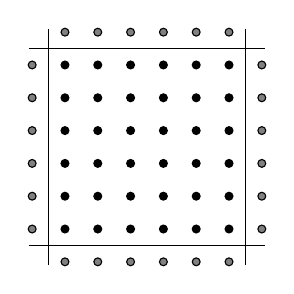
\begin{tikzpicture}[scale=2.5]
			\draw (-0.1,0) --(1.1,0);
			\draw (0, -0.1) -- (0, 1.1);
			\draw(-0.1, 1) -- (1.1, 1);
			\draw(1, -0.1) -- (1, 1.1);
			%Interior gridpoints
			\foreach \x in {0,...,5}
			\foreach \y in {0,...,5}
			{\draw[fill=black] ((\x/6 + 1/12, \y/6+1/12) circle (0.02);}
			\foreach \x in {0,...,5}
			{\draw[fill=gray] (-1/12, \x/6+1/12) circle (0.02);
				\draw[fill=gray] (13/12, \x/6+1/12) circle (0.02);
				\draw[fill=gray] (\x/6+1/12, -1/12) circle (0.02);
				\draw[fill=gray] (\x/6+1/12, 13/12) circle (0.02);}
			\end{tikzpicture}
		\end{center}
		\caption{\label{fig:resid-overlap} The nodes used in computing the residual for a square domain.  The nodes in gray are stored on other processors and must be communicated.}
	\end{figure}
	
	The fact that each grid point is contained in only one domain simplifies computations (since this means that updates are entirely local, rather than depending on computations from several neighboring processors).  However, the analytic grids can be seen to have an overlap of size \(h\) (see Figure~\ref{fig:min-overlap}).  This minimal overlap is remarked on in Chapter 1 of~\cite{Dolean15}.
	
	\begin{figure}
		\begin{center}
			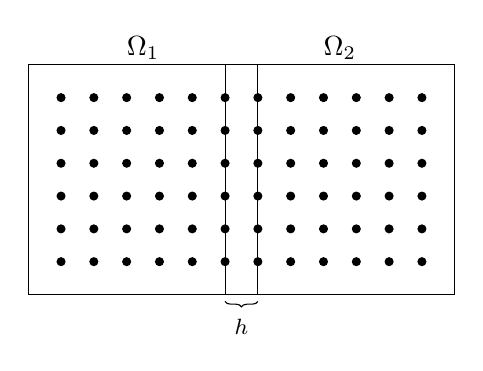
\begin{tikzpicture}[scale=2.5]
			\draw (-1/12,-1/12) -- (-1/12, 13/12) -- (13/12, 13/12) -- (13/12, -1/12) -- (-1/12, -1/12);
			\draw (11/12,-1/12) -- (11/12, 13/12) -- (25/12, 13/12) -- (25/12, -1/12) -- (11/12, -1/12);
			\foreach \x in {0,...,5}
			\foreach \y in {0,...,5}
			{\draw[fill=black] ((\x/6 + 1/12, \y/6+1/12) circle (0.02);
				\draw[fill=black] ((\x/6 + 13/12, \y/6+1/12) circle (0.02);}
			\draw [decorate,decoration={brace,amplitude=2pt},xshift=0pt,yshift=-1pt] (13/12,-1/12) -- (11/12,-1/12) 
			node [black,midway, yshift=-9pt] {\footnotesize $h$};
			\node at (0.5, 7/6) {$\Omega_1$};
			\node at (1.5, 7/6) {$\Omega_2$};
			\end{tikzpicture}
			\caption{\label{fig:min-overlap} The overlap between two adjacent domains is order \(h\).}
		\end{center}
	\end{figure}
	
	\section{Scaling results}
	\textbf{Weak Scaling}: The local grid is fixed to be $100\times100$ and the number of processors are assumed to be a perfect square with $max iter=500$. 
	
	\includegraphics[scale=.4]{/Users/sanchit/Desktop/high_performace_computing/repository/finalproj/weak_scaling.jpg}
	
	As is evident from the plot the problem scales well. The increase in time is mostly because of increased communication because we are using a local solver(UMFPACK) to solve the poisson's equation locally which works in the same time as the local problem size is fixed.
	
	\textbf{Strong Scaling}: The global grid is fixed at $3600\times3600$ and the number of processors are assumed to be a perfect square with $max iter=100$.
	
	\includegraphics[scale=.4]{/Users/sanchit/Desktop/high_performace_computing/repository/finalproj/strong_scaling.jpg}

The plot suggests that the problem scales strongly almost perfectly. 
	\section{Possible improvements}
	\begin{itemize}
\item	The strong scaling demonstrates that the convergence is very slow, both in time and in residual as well. This is in agreement with the theory that suggesgs that the converence is proportional to the overlap between the domains. So a possible improvement would be to implement the code that can tackle the overlapping domains. 
\item Another possible direction to improve would be to coupling the multigrid or multilevel methods to get a better convergence rate.
\item Nonoverlapping method can be used as a preconditioner for GMRES or CG, so exploring this direction is another option for future studies.
	\end{itemize}

	\section{Author contributions}
	
	Gavin Stewart wrote the part of the algorithm which computes local corrections, and the sections `Introduction' and `The Algorithm' of the report.  Sanchit Chaturvedi wrote the part of the algorithm which computes the residuals and global residual norms, and the sections `Scaling results' and `Possible improvements.'  Both authors contributed to the debugging of the code.
	
	\begin{thebibliography}{9}
		\bibitem{Davis04}
		Davis, T.A.
		(2004).
		\emph{Algorithm 832: UMFPACK V4.3--an unsymmetric-pattern multifrontal method}.
		ACM Transactions on Mathematical Software (TOMS)
		30(2), 196 -- 199.
		
		\bibitem{Dolean15}
		Dolean, V., Jolivet, P., \& Nataf, F.
		(2015).
		\emph{An Introduction to Domain Decomposition Methods: Algorithms, Theory, and Parallel Implementation}.
		SIAM, Philadelphia.
		
		\bibitem{Fairweather03}
		Fairweather, G., Karageorghis, A., \& Martin, P.A.
		(2003).
		\emph{The method of fundamental solutions for scattering and radiation problems}.
		Engineering analysis with boundary elements   
		27(7), 759--769.
		\url{https://doi.org/10.1016/S0955-7997(03)00017-1}
		
		\bibitem{Marshall97}
		Marshall, J., Adcroft, A., Hill, C., Perelman, L., \& Heisey, C.
		(1997).
		\emph{A finite-volume, incompressible Navier Stokes model for studies of the ocean on parallel computers}.
		Journal of Geophysical Research 
		102(C3), 5753--5766.
		
	\end{thebibliography}
\end{document}